\documentclass[10pt,letterpaper]{article}
% Add a bunch of useful math, font, and symbols
\usepackage{amsfonts}
\usepackage{amsmath}
\usepackage{amssymb}

% English support
\usepackage[english]{babel}

% Citation
\usepackage[superscript]{cite}

% Better enumerate and itemize
\usepackage{enumitem}

% Better control of headers and footers
\usepackage{fancyhdr}

% Floating objects like figures and tables
\usepackage{float}

% Page layout and dimensioning
\usepackage[margin=1in]{geometry}

% Basic color, graphics and text manipulation 
\usepackage{graphicx}

% Use Helvetica typeface
\usepackage[scaled]{helvet}
\renewcommand\familydefault{\sfdefault} 
\usepackage[T1]{fontenc}

% Cross-referencing hyperlinks
\usepackage{hyperref}

% Line break for long URLs
\usepackage{breakurl}

% Accept utf-8 input encoding
\usepackage[utf8]{inputenc}

% Make indexes
\usepackage{makeidx}

% Microtype (apparently makes the typographics stuff better)
\usepackage{microtype}

% [Disabled] multi-column writing
% \usepackage{multicol}

% English ordinal counting (1st, 2nd, etc.)
\usepackage{nth}

% Long table
\usepackage{longtable}

% Paragraph skip - adds extra lineskip spacing
\usepackage{parskip}
\setlength{\parskip}{0.7\baselineskip plus 2pt}

% Add ability to set space between lines
\usepackage{setspace}

% S.I. units
\usepackage{siunitx}

% Subcaptions for subfigures
\usepackage{subcaption}

% Include svg graphics
\usepackage{svg}

% Drawing graphics
\usepackage{tikz}

% Subsubsubsection
\usepackage{titlesec}
\setcounter{secnumdepth}{4}
\titleformat{\paragraph}
{\normalfont\normalsize\bfseries}{\theparagraph}{1em}{}
\titlespacing*{\paragraph}
{0pt}{3.25ex plus 1ex minus .2ex}{1.5ex plus .2ex}

% Custom titles
\usepackage{titling}

% Url
\usepackage{url}

\RequirePackage[figure,table]{totalcount}


% Custom definitions
\newcommand{\doctitle}{Validation Specification}
\newcommand{\docsubtitle}{Computing Platform Multirotor with FPGA Hardware Acceleration Applications}

% Custom commands
\newcommand{\ts}{\textsubscript}	% Subscript command %


% Use hyphans to break up urls
\def\UrlBreaks{\do\/\do-}

% PDF and href setup
% Hyper ref
\hypersetup{
	colorlinks=true,
	citecolor=black,
	linkcolor=black,
	filecolor=black,
	urlcolor=blue,
	pdftitle={\@title},
	bookmarks=true
}
\urlstyle{same}
% Page headings
\pagestyle{fancy}
\fancyhead[L]{\MakeUppercase{CPEN/ELEC 491}}
\fancyhead[C]{\textbf{\doctitle}}
\fancyhead[R]{Mieszko Lis, PhD}
\fancyfoot{}
\fancyfoot[C]{Non-Confidential}
\fancyfoot[R]{\thepage}

% No paragraph indent
\parindent 0ex

% Meta
\author{
	Deutsch, Peter &
	\textit{me@peterdeutsch.ca}
	\\
	He, Muchen &
	\textit{m.he@alumni.ubc.ca}
	\\
	Hsueh, Arthur &
	\textit{ah11962@outlook.com}
	\\
	Wang, Meng &
	\textit{wzfftxwd@gmail.com}
	\\
	Wilson, Ardell &
	\textit{ardellw96@gmail.com}
}
\title{\doctitle}
\date{\today}
\makeatletter
\renewcommand{\maketitle}{
	\bgroup
	\setlength{\parindent}{0pt}
	\begin{flushleft}
		% Top spacing
		\vspace*{0.5in}

		% Team logo
		
\includegraphics[scale=0.4]{../assets/capstonelogo1.png}
		\vspace*{0.25in}

		% Title
		\textbf{\Huge{\@title}}\\
		\hrulefill

		% Subtitle
		\textbf{\huge{\docsubtitle}}
		
		\vspace*{0.5in}

		% Course number and team
		\textbf{\Large{CPEN/ELEC 491 Capstone Team 109}}\\
		\hspace*{0.1cm}
		\begin{tabular}[h]{|ll}
			\@author
		\end{tabular}

		\vspace*{0.25in}

		\textbf{\Large{Mieszko Lis, PhD}}\\
		\hspace*{0.1cm}
		\begin{tabular}[h]{|ll}
			Electrical and Computer Engineering, The University of British Columbia
		\end{tabular}

		\vfill
		
		% Date
		\large{Revision 1.0 -- \@date}
		\vspace*{0.5in}

		% Logo
		\hspace*{-0.3cm}
\includegraphics[scale=0.5]{../assets/ece_logo.pdf}

	\end{flushleft}
	\egroup
}
\makeatother

% Begin Document
\begin{document}

% Title Page
\begin{titlepage}
	\maketitle
\end{titlepage}


\renewcommand{\thepage}{\roman{page}}
\setcounter{page}{1}

% Revision history
\backgroundsetup{
	scale=1,
	color=black,
	opacity=0.3,
	angle=0,
	contents={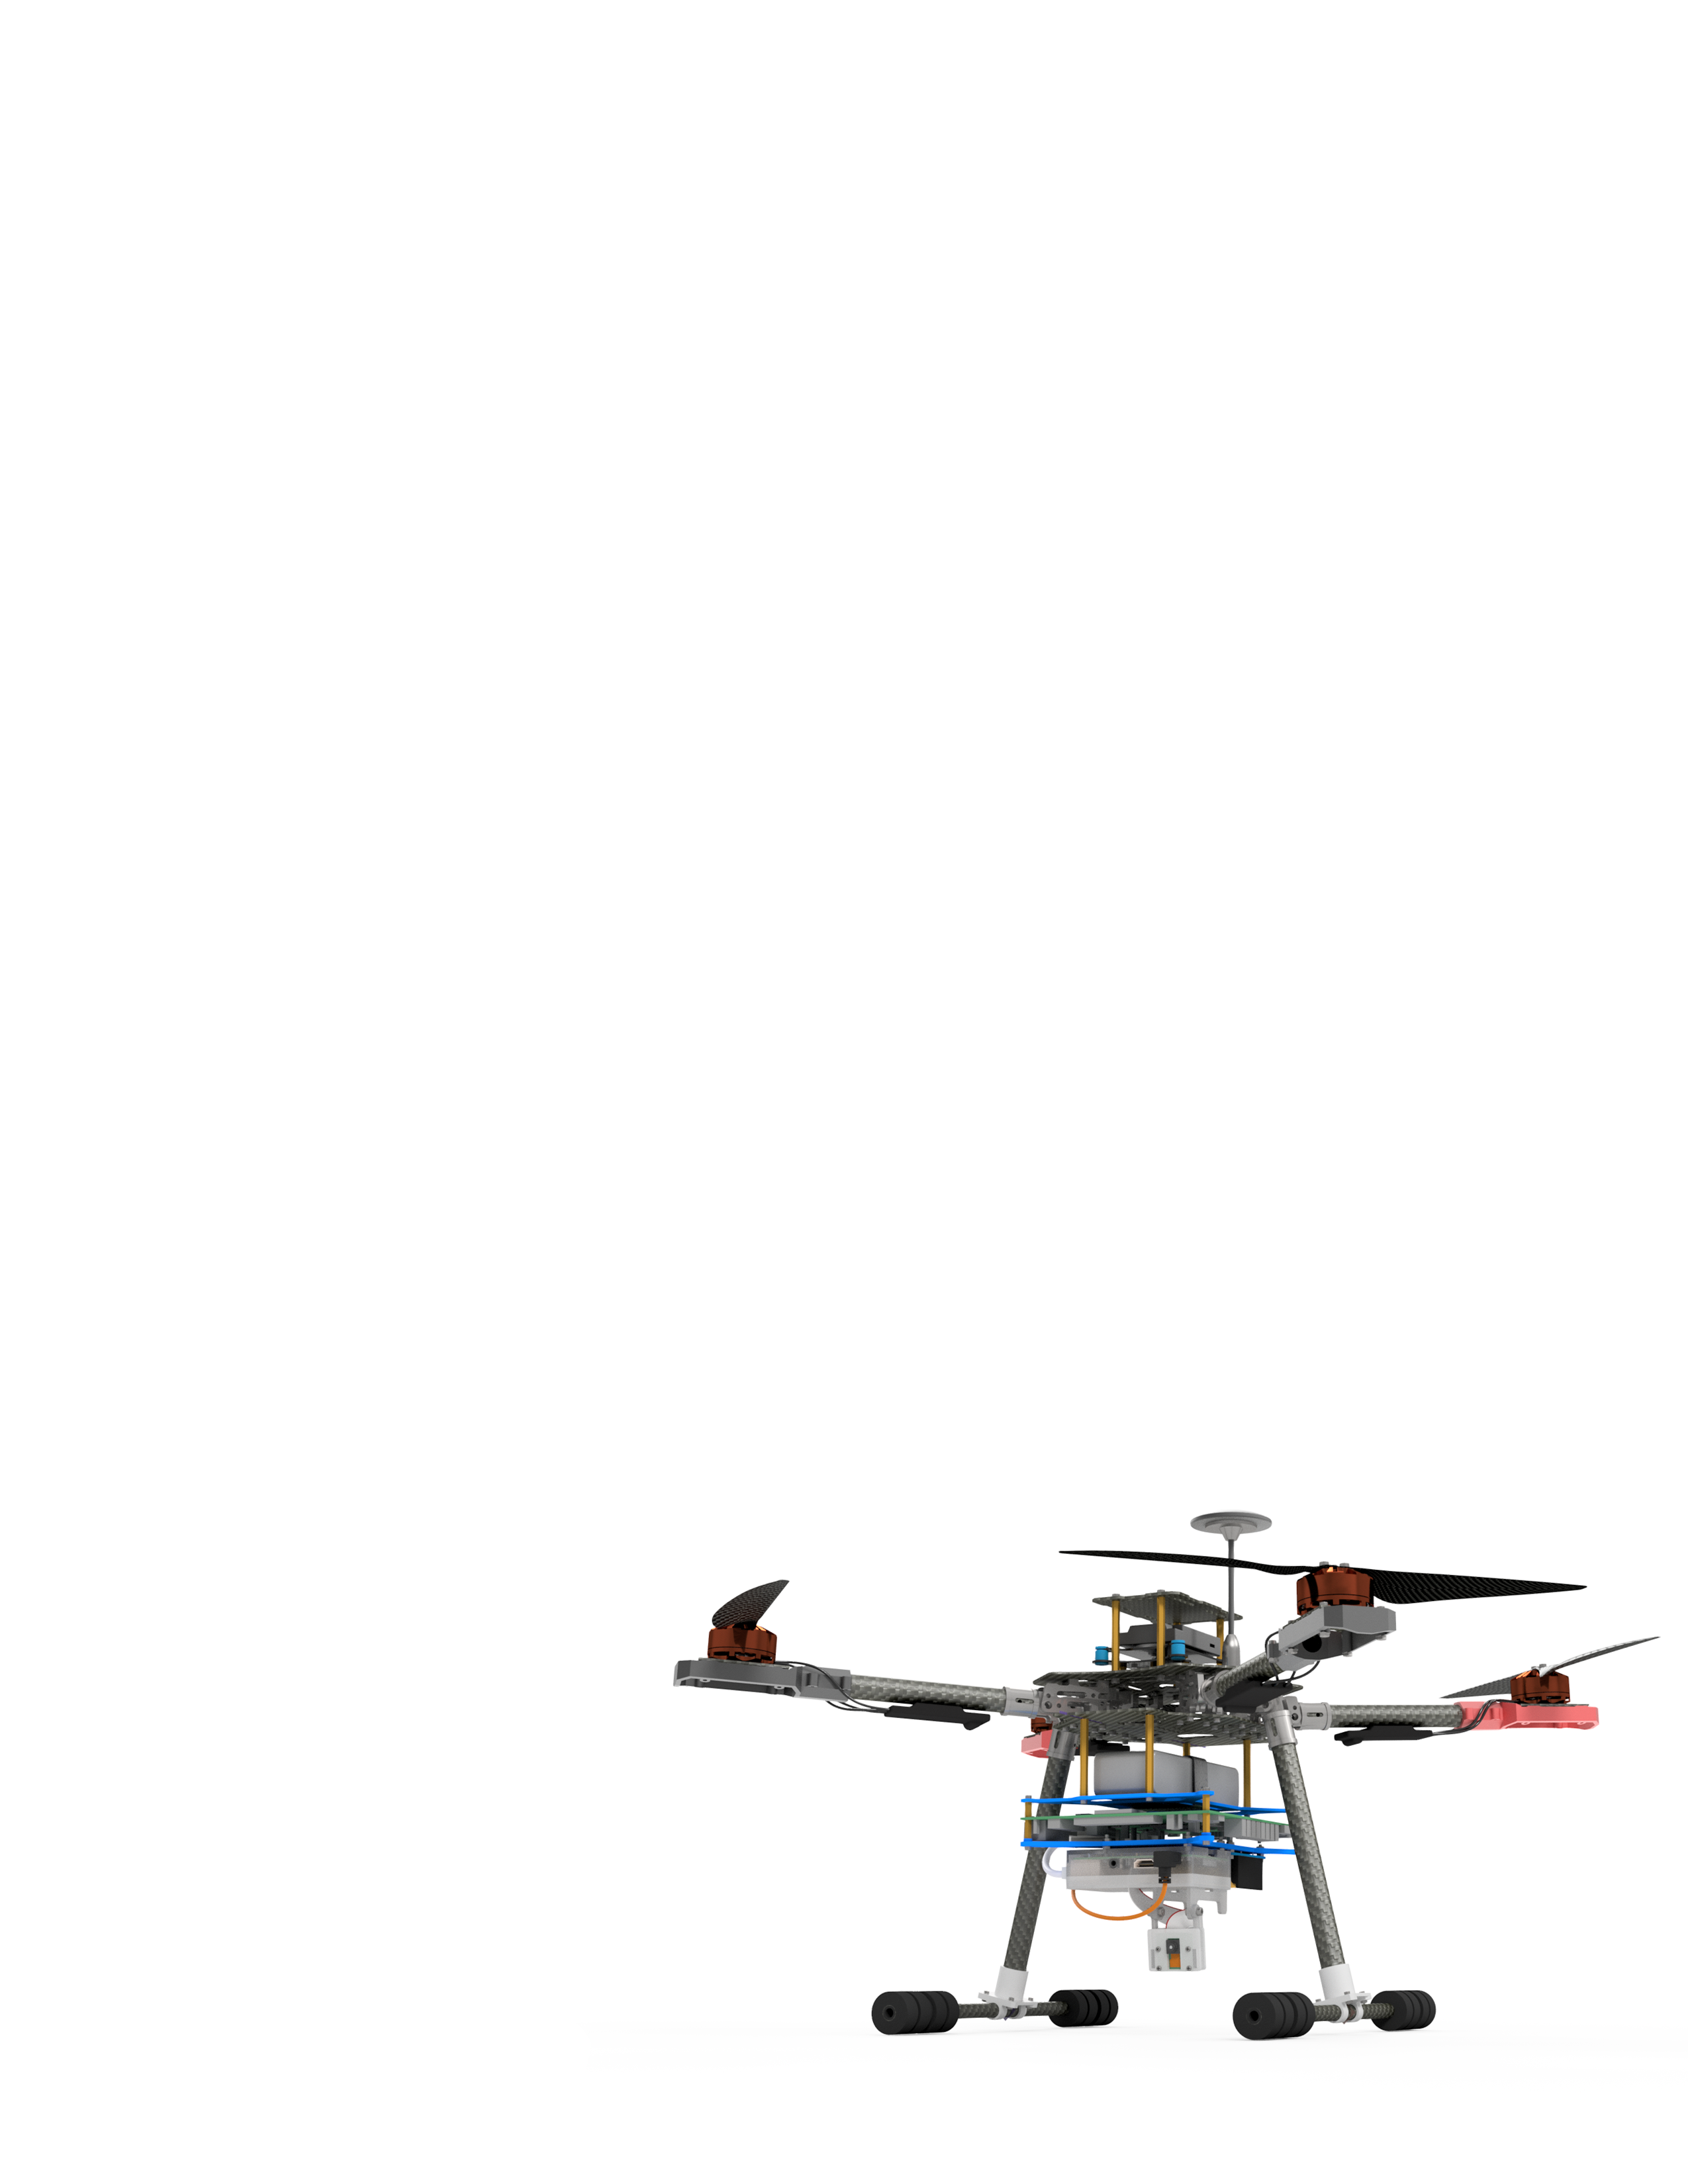
\includegraphics[height=\paperheight,width=\paperwidth]{../assets/render2bg}}
}
\BgThispage
%\thispagestyle{empty}
\section*{Revision History}
The full revision history and commited changes of the document can be found in the git repository history: \href{https://github.com/Capstone-Skynet/Capstone-Skynet.github.io}{https://github.com/Capstone-Skynet/Capstone-Skynet.github.io/commits/master}.

\begin{table}[H]
\begin{tabular}{*{4}{l}p{0.5\linewidth}}
\hline
Version \# & Initials & Release Date & Changeset & Changes Made \\ \hline

0.0 & PD & 2019-10-11 & \texttt{660e001} & Initial skeleton of the document.\\
0.1 & MH & 2019-10-11 & \texttt{6af9e8a} & Populate initial document with draft content required for Milestone I.\\
0.2 & PD & 2019-11-23 & & Initial framework for test descriptions created.\\
0.3 & MW & 2019-11-24 & & First set of tests added.\\
1.0 & PD & 2019-11-25 & & General clean-up and release for Milestone II.\\
1.1 & AH & 2020-02-09 & & Added Full System Tests \\

 & & & \\ \hline
\end{tabular}
\end{table}
\clearpage

% Table of contents
\setcounter{secnumdepth}{3}
\tableofcontents

% Roman numeral page numbers


% Terms and Abbreviations
\thispagestyle{empty}

\section*{Terms and Abbreviations}

Technical terms and abbreviations dictionary go here.

\begin{tabular}[h]{rp{0.75\linewidth}}
    \hline
    \textbf{Term} & \textbf{Definition}\\
    \hline

    ANN & Artificial Neural Network, or simply ``Neural Network'', is a data processing model modeled after neuron interactions. The process consists of forward propagation using several matrix multiplications.\cite{ann}\\
    ASIC & Application-specific Integrated Circuits.\\
    CNN & Convolutional neural network are neural networks that is especially useful for image classification.\cite{cnn} \\
    ECE & Department of Electrical and Computer Engineering at the University of British Columbia.\\
    FPGA & Field-Programmable-Gate-Arrays, ``programmable'' hardware that allows ASIC-like performance with software-like turn-around time and flexibility.\\
    GPU & Graphics Processing Unit, a discrete piece of hardware designed to accelerate graphic-intensive or other parallel computing tasks.\\
    LOS & Line-of-sight.\\
    ML & Machine learning.\\
    Multirotor & An unmanned vehicle with multiple engines. \\
    OTS & Off-the-shelf, or commercially available/purchasable \\
    PID / PID Controller & Proportion-Integral-Derivative controllers is the most common control algorithm for precise and accurate movement, as well as to compensate external forces.\cite{pid}\\
    RNN & Recurrent neural networks are neural networks where the output depends on previous computations, essentially consists of memory.\cite{rnn}\\
    RX & Receiver.\\
    TC & Transport Canada.\\
    TX & Transmitter.\\
    YOLO & You-Only-Look-Once is a fast ML algorithm that detect objects but is unlike CNN nor RNN.\cite{yolo}\cite{yolo-2}\\
     & \\

    \hline

\end{tabular}


% List of figures and tables
\iftotalfigures
\addcontentsline{toc}{section}{\listfigurename}
\listoffigures
\fi
\iftotaltables
\addcontentsline{toc}{section}{\listtablename}
\listoftables
\fi

\newpage

% Set page and section counter
\renewcommand{\thepage}{\arabic{page}}
\setcounter{page}{1}



% TODO: fill out all the sections
% if the sections gets too long, move them to a separte .tex document
\section{About This Document}

\subsection{Purpose}
This document serves to outline the methods, tests, and scenarios which are used to validate the project, and the status of these validation steps. In addition, this document outlines the validation methodology, which describes how the validation steps themselves are written and performed.

\subsection{Intended Audience}
This document is intended for:
\begin{itemize}
\item \textbf{Quality Controllers (the Capstone team)}: to assess the validation methodology and results,
\item \textbf{Designers (the Capstone team)}: to assess the current degree of completion of the project,
\item \textbf{Client (and their representatives)}: to assess the final state of the project (when complete),
\item \textbf{and Legal Personnel:} to review the validation scheme if necessary. Such personnel may include individuals from the Department of Electrical and Computer Engineering, Industry Canada, and Transport Canada.
\end{itemize}

This document is particularly relevant to those who wish to assess the current state of the project, in addition to those who will assess the validation methodology against academic, organizational, or legal criteria.

\subsection{Reading Guide}
This document begins with a description of the validation methodology, describing differing types of tests and how they are identified. The description of tests begins in Section \ref{begintest}, with each test case listing the requirements being tested, the steps taken to execute the test, and the test's success parameters. Finally, the current status of each test is summarized in Section \ref{results}. Any pertinent test results are additionally included as appendices, as appropriate.

The requirements referenced in this document can be found in the \textit{Requirements Specification}.

\section{Validation Overview}

\subsection{Test Organization}\label{auto}
The validation tests employed are split into two categories: \textit{automated tests} and \textit{manual tests}:

\textbf{Automated tests} are tests focused on tasks which are performed regularly by the device and \textit{can be monitored by the device itself}. Examples of such tests include self-tests on boot, self-monitoring of communication status, machine learning accuracy logging, et cetera.

\textbf{Manual tests} are tests which \textit{cannot be performed by the device itself} and must be manually performed by a quality controller. These tests are performed less frequently --- some may be executed before every flight, while others may only be performed once. 

\subsection{Test Notation}
The following notations and conventions are used throughout this document:

\textbf{Verification Requirement (VR)}: The unique identifier of a specific test. These identifiers always start with \textbf{T}.

\textbf{Design Requirement (DR)}: Denotes the design requirement which the test is exercising, as listed in the project's \textit{Requirements Specification}. Requirement identifiers are encoded by their first characters, as follows:
\begin{itemize}
	\item \textbf{F}: Functional Requirement,
	\item \textbf{NF}: Non-Functional Requirement, and
	\item \textbf{C}: Constraint
\end{itemize}

\textbf{Status}: The status of a specific test:
\begin{itemize}
	\item \textbf{PEND} if the specific test has never been performed,
	\item \textbf{FAIL} if the specific test is currently failing, or
	\item \textbf{PASS} if the specific test is currently passing
\end{itemize}

\textbf{Effective Date}: Denotes the date at which the test was last performed (and thus, when the status was last updated). This field is not applicable for pending tests.

\textbf{It is important to note that a one-to-one mapping of VRs to DRs \textit{does not necessarily exist}}. Some requirements (particularly those which are high-level or functional) will have no tests, while some requirements will have multiple tests. It is also possible for one test to exercise multiple design requirements at once.

\section{Automated Test Cases} \label{begintest}

%\subsection{Computing Platform Tests}
\paragraph{\underline{T.ACP.1: Wireless Connection Checking}}

This test is performed automatically after system boot to confirm that the wireless connection between the Raspberry Pi and the ground station has been established.

\textbf{Addresses}: F.CM.1, F.CM.2, F.BS.3, F.BS.5

\textbf{Procedure}:
\begin{enumerate}[noitemsep]
    \item The platform management board sends a test string to the base station.
    \item The base station echos back the string.
    \item The platform management board verifies the result.
\end{enumerate}

\textbf{Verification}: 
Upon successful completion, the base station displays a message to indicate successful connection and live video streaming will be displayed on the screen.

%\subsection{Multirotor Tests}
%\input{3_2_automated_multirotor_test.tex}

\section{Manual Test Cases}

\subsection{Computing Platform Tests}
\subsubsection{General Tests}
\paragraph{T.G.1: System Boot Test}

This test verifies the system can boot to an operational ready stage.

\textbf{Addresses}: F.CP.2

\textbf{Procedure}:
\begin{enumerate}[noitemsep]
    \item Setup all prerequisites the system requires, i.e. power cable is connected.
    \item Boot up the system.
    \item Connect the base station to the server.
    \item Wait for the status message showed up on the base station.
\end{enumerate}

\textbf{Verification}: 
If a warning/error message or no message is received on the base station after 5 minus, that's an indication of a failed test. Otherwise, the test is passed.

%

\paragraph{T.G.2: System Logging Test}

This test triggers a system fault and verifies the error message is correctly displayed and the log data is correctly recorded.

\textbf{Addresses}: F.CP.4, F.BS.5

\textbf{Procedure}:
\begin{enumerate}[noitemsep]
    \item Turn off the Wi-Fi router that the Raspberry Pi is trying to connect to.
    \item Boot the system.
    \item Let the system run 5 minutes.
    \item Verify the system displayed message and the log file the Raspberry Pi creates.
\end{enumerate}

\textbf{Verification}: 
There should have an error message display on the base station. The log file should clearly indicate that the system couldn't connect to the router and tried to reconnect. If the error message is correctly displayed and the file is correctly generated, this test is passed.

%

\paragraph{T.G.3: Wireless Connection Test}

This test verifies the effective range of the wireless connection between the Raspberry Pi.

\textbf{Addresses}: F.BS.3, NF.CM.1, NF.CM.2

\textbf{Procedure}:
\begin{enumerate}[noitemsep]
    \item Place the Raspberry Pi, the base station, and the Wi-Fi router at vertices of an equilateral triangle with side length of 30 meters.
    \item Write a video streaming application.
    \item Streaming the video on the Raspberry Pi.
    \item Check the streaming quality on the base station.
\end{enumerate}

\textbf{Verification}: 
A stable connection refers to no obvious lost of frames can be noticed on the base station.

\subsubsection{Camera Tests}
\paragraph{T.CM.1: Camera Test}

This test verifies the attributes of the video that captured by the camera.

\textbf{Addresses}: NF.CAM.3, NF.CAM.4

\textbf{Procedure}:
\begin{enumerate}[noitemsep]
    \item The Raspberry Pi stores a 10-second video sample.
    \item Verify the video attributes on the Raspberry Pi.
\end{enumerate}

\textbf{Verification}: 
Compare the resolution and frame rate of the stored video with the setting.

%

\paragraph{T.CM.2: Camera Focusing Test}

This test verifies the camera's auto focus functionality.

\textbf{Addresses}: NF.CAM.1, NF.CAM.2

\textbf{Procedure}:
\begin{enumerate}[noitemsep]
    \item Place a testing object 10 meters away from the camera.
    \item Clear objects that is between the camera and the testing object.
    \item Take a picture using the camera with default setting.
\end{enumerate}

\textbf{Verification}: 
The focus should be on the testing object, that is, the testing object should be easily identified in the image.

%

\paragraph{T.CM.3: Video Recording Test}

This test verifies the video captured by camera can be stored into a video file.

\textbf{Addresses}: F.CAM.2, NF.CAM.6

\textbf{Procedure}:
\begin{enumerate}[noitemsep]
    \item Turn on the camera.
    \item Start recording for two hours.
\end{enumerate}

\textbf{Verification}: 
Verify that the recorded video file can be played back.

%

\paragraph{T.CM.4: Various Light Condition Camera Test}

This test verifies the automatic exposure functionality of the camera.

\textbf{Addresses}: NF.CAM.5

\textbf{Procedure}:
\begin{enumerate}[noitemsep]
    \item Select 5 different time in a day with different light conditions.
    \item Recording a 1-minute video at each of the selecting time at the same place.
\end{enumerate}

\textbf{Verification}: 
Verify that the objects in the recorded video can be easily identified.

\subsubsection{Machine Learning Tests}
\paragraph{\underline{T.ML.1: ML Sample Image Test}}

This test checks if the ML model accelerator accurately generates bounding boxes for images within the official sample collection provided by the YOLOv2 authors.

\textbf{Addresses}: F.ML.1, F.ML.4

\textbf{Procedure}:
\begin{enumerate}[noitemsep]
    \item Manually transfer a sample image to the PLB via a file-transfer protocol.
    \item Directly call the ML helper function which communicates with the hardware accelerator core.
    \item Manually verify the results for correctness.
\end{enumerate}

\textbf{Verification}: 
Confirm visually that objects in the sample image are accurately identified and bounded.

\paragraph{\underline{T.ML.2: ML Video Results Test}}

This test verifies the correctness of the ML results.

\textbf{Addresses}: F.HL.2, F.ML.1, F.ML.4

\textbf{Procedure}:
\begin{enumerate}[noitemsep]
    \item Prepare a test video with pre-labelled results.
    \item Feed the test video to the machine learning model.
    \item Record the results from the machine learning model.
\end{enumerate}

\textbf{Verification}: 
Verify that the ML results match with the pre-labelled results.

%
\paragraph{\underline{T.ML.3: ML Latency Test}}

This test checks if the latency of the machine learning model is acceptable.

\textbf{Addresses}: F.ML.3

\textbf{Procedure}:
\begin{enumerate}[noitemsep]
    \item Write a program to record the timestamp for each processed frame received on the PMB.
    \item Calculate the timing gaps between 100 consecutive frames.
\end{enumerate}

\textbf{Verification}: 
Confirm that there are no frame gaps greater than one second.

\subsubsection{Base Station Tests}
\paragraph{T.BS.1: Video Content Test}

This test checks the integrity of the transmitted video.

\textbf{Addresses}: F.CM.1, F.CP.1

\textbf{Procedure}:
\begin{enumerate}[noitemsep]
    \item Save a 1-minute video sample and ML results on the Raspberry Pi.
    \item Have a screen recording on the base station at the same time.
\end{enumerate}

\textbf{Verification}: 
If no visible difference can be detected between the two video footage, the test is passed.

\subsubsection{Power Tests}
\paragraph{\underline{T.P.1: Power Usage Test}}

This test checks actual power usage of the system.

\textbf{Addresses}: NF.PR.1

\textbf{Procedure}:
\begin{enumerate}[noitemsep]
    \item Setup the system in the lab.
    \item Power the Raspberry Pi and the FPGA board using two power supplies.
    \item Boot the system and start the machine learning implementation.
    \item Record the power reading (voltage and current).
\end{enumerate}

\textbf{Verification}: 
Compare the peak power with the maximum power listed in the user manual. If the recorded peak power does not exceed the theoretical maximum power, the test passes. 

%

\paragraph{\underline{T.P.2: Battery Safety Test}}

This test verifies the functionality of the battery protection circuit.

\textbf{Addresses}: F.PR.4, F.PR.5, F.PR.6

\textbf{Procedure}:
\begin{enumerate}[noitemsep]
    \item Connect the battery protection circuit to a lab power supply.
    \item Load it with an appropriately sized resistor in order to simulate normal operating conditions.
    \item Raise the supply voltage and probe the output voltage in order to verify that our overvoltage protection works correctly.
    \item Connect the supply voltage in backwards in order to verify that the reverse polarity protection works correctly.
\end{enumerate}

\textbf{Verification}: 
If sparking or overheating occurs during the test, then the test has failed.

\paragraph{\underline{T.P.3: Computing Platform Battery Test}}

This is a battery life test and it also verifies the stability of the supply voltage when the battery is not fully charged.

\textbf{Addresses}: F.PR.1, F.PR.4

\textbf{Procedure}:
\begin{enumerate}[noitemsep]
    \item Fully charge the battery.
    \item Breakout the battery to connect the multimeter to its output port.
    \item Record the voltage reading of the fully charged battery. 
    \item Connect the PMB and PLB to the battery and power up.
    \item Launch two testing program on both boards and let it run for 30 minutes.
    \item Record the voltage reading and current reading every minute.
    \item Power off the PMB and PLB and record the after-test voltage reading and battery level.
\end{enumerate}

\textbf{Verification}: 
To ensure a minimum of 30 minutes of operation time, the after-test battery level must be at least 50\%. The voltage drop must be within 2V to ensure a stable power output to the PMB and PLB.


\subsection{Multirotor Tests}
\paragraph{T.DR.1: RPAS Maximum Takeoff Weight Test}

This test obtains the maximum thrust output, minimum thrust-to-weight ratio, and maximum power output of the RPAS prototype.

\textbf{Addresses}:  NF.DR.1, NF.DR.12, NF.DR.13

\textbf{Procedure}:
\begin{enumerate}[noitemsep]
    \item Attach the RPAS prototype to a scale or force sensor and ensure that the RPAS cannot separate scale or force sensor.
    \item Attach multimeter to the RPAS power circuitry.
    \item Fix or constrain the RPAS to the ground by using a heavy weight, tape, or fasteners.
    \item Tare the scale or force-sensor such that the measure is reference to the initial conditions.
    \item Power on the drone and arm the motors.
    \item Apply maximum throttle from the radio transmitter.
    \item Obtain voltage and current measurements from the multimeter.
    \item Obtain force measurements from the scale or force sensor.
\end{enumerate}

\textbf{Verification}: 
To ensure that the RPAS has minimum manuverability, at maximum take-off weight, we should be using 80\% throttle. For this test to pass, the RPAS must achieve a maximum pull of 125\% (2.5 kg) of maximum takeoff weight. Since this is a maximum load test case, we verify the measured current and voltage to ensure NF.DR.12 and NF.DR.13 are checked.

% 

\paragraph{T.DR.2: RPAS Typical Takeoff Weight Test}

The typical takeoff weight test quantifies the flight-time of the RPAS during a typical operation with significantly less massive payload.

\textbf{Addresses}: NF.DR.7, NF.DR.10

\textbf{Procedure}:
\begin{enumerate}[noitemsep]
    \item Attach voltage and current monitor to the RPAS power circuitry.
    \item Set up RPAS for test-flight in open area or large room.
    \item Power on the drone and arm the motors.
    \item Start timer.
    \item Apply reasonable throttle from the radio transmitter such that the RPAS is hovering 3.0 m above ground.
    \item Record the \%-throttle applied for hovering.
    \item Keep hovering until the RPAS battery reaches 10\% capacity.
    \item Stop timer when the RPAS lands; calculate flight time in minutes.
    \item Measure the total mass of the RPAS and payload, and compute the average power consumption using the data acquired from the voltage and current monitors. Calculate efficiency in g/W.
\end{enumerate}

\textbf{Verification}:
The measured flight time should be greater than 20 minutes with a payload mass of 500 g in order to satisfy the requirement NF.DR.7. The calculated efficiency must be greater than 5.0 g/W to satisfy the requirement NF.DR.10.

\subsection{Full System Tests}
\paragraph{\underline{T.FS.1: Full System Flight Test}}

This test verifies the flight capability of the fully integrated system.

\textbf{Addresses}: F.HL.1

\textbf{Procedure}:
\begin{enumerate}[noitemsep]
    \item Turn on the computing platform, ensuring the PMB and PLB are secured on the RPAS.
    \item Using the RPAS controller, direct the RPAS to rise from its ground position to a comfortable flight height.
    \item Using the RPAS controller, direct the RPAS to move horizontally in a wide range of directions.
    \item Using the RPAS controller, direct the RPAS to land back on the ground.
\end{enumerate}

\textbf{Verification}:
Confirm that the RPAS, mounted with the PMB and PLB, is capable of lifting off, flying in all directions and landing safely down on the ground.

%

\paragraph{\underline{T.FS.2: Full System ML Processing Test}}

This test verifies the ML processing capability of the fully integrated system.

\textbf{Addresses}: F.HL.2, F.HL.3, F.HL.4

\textbf{Procedure}:
\begin{enumerate}[noitemsep]
    \item Turn on the computing platform, ensuring the PMB and PLB are secured on the RPAS.
    \item Using the RPAS controller, direct to RPAS to rise from its ground position to a comfortable flight height.
    \item Check the base station interface to ensure there is real-time video and ML data being displayed.
\end{enumerate}

\textbf{Verification}:
Confirm that the fully integrated system is capable of ML processing, from taking in captured video on the PMB to displaying accurate ML data and captured video on the base station.

\section{Verification Results} \label{results}

\subsection{Automated Verification Results}
\begin{table}[H]
	\centering
	\begin{tabular}{lllll}
	\hline
	\textbf{VR} & \textbf{DR} & \textbf{Status} & \textbf{Eff. Date} & \textbf{Note}\\
	\hline
	T.ACP.1 & F.CM.1, F.CM.2, F.BS.3, F.BS.5 & PEND   & \\
	T.ACP.2 & NF.CP.1, F.ML.1, F.ML.2, F.ML.4 & PEND   & \\
	\hline
	\end{tabular}
\end{table}

\subsection{Manual Verification Results}
\subsubsection{Computing Platform Verification Results}
\begin{table}[H]
	\centering
	\begin{tabular}{lllll}
	\hline
	\textbf{VR} & \textbf{DR} & \textbf{Status} & \textbf{Eff. Date} & \textbf{Note}\\
	\hline
	T.G.1 & F.CP.2 & PEND   & \\
	T.G.2 & F.CP.4, F.BS.5 & PEND   & \\
	T.G.3 & F.BS.3, NF.CM.1, NF.CM.2 & FAIL   & 24-JAN-20 & Wi-Fi range is \textasciitilde 10m, need to add a Wi-Fi antenna. \\
	\hline
	T.CM.1 & NF.CAM.3, NF.CAM.4   & PEND   & \\
	T.CM.2 & NF.CAM.1, NF.CAM.2   & PEND   & \\
	T.CM.3 & F.CAM.2, NF.CAM.6   & PEND   & \\
	T.CM.4 & NF.CAM.5   & PEND   & \\
	\hline
	T.ML.1 & F.ML.1, F.ML.4 & PASS & 3-FEB-20 & See Appendix \ref{appendix:T.ML.1}.\\
	T.ML.2 & F.HL.2, F.ML.1, F.ML.4 & FAIL  & 5-FEB-20 & FPS is currently \textasciitilde 0.33, need to optimize data flow. \\
    T.ML.3 & F.ML.3 & PEND   & \\
    \hline
    T.BS.1 & F.CM.1, F.CP.1 & PEND   & \\
    \hline
    T.P.1 & NF.PR.1 & PASS   & 1-FEB-20 & See Appendix \ref{appendix:T.P.1}.\\
    T.P.2 & F.PR.4, F.PR.5, F.PR.6 & PEND   & \\
    T.P.3 & F.PR.1, F.PR.4 & PASS   & 30-JAN-20 & See Appendix \ref{appendix:T.P.3}. \\
	\hline
	\end{tabular}
\end{table}

\subsubsection{Multirotor Verification Results}
\begin{table}[H]
	\centering
	\begin{tabular}{lllll}
	\hline
	\textbf{VR} & \textbf{DR} & \textbf{Status} & \textbf{Eff. Date} & \textbf{Note}\\
	\hline
    T.DR.1 & NF.DR.1, NF.DR.12, NF.DR.13  & PEND   & \\
	T.DR.2 & NF.DR.7, NF.DR.10 & PEND   & \\
	\hline
	\end{tabular}
\end{table}

\subsubsection{Full System Verification Results}
\begin{table}[H]
	\centering
	\begin{tabular}{lllll}
	\hline
	\textbf{VR} & \textbf{DR} & \textbf{Status} & \textbf{Eff. Date} & \textbf{Note}\\
	\hline
    T.FS.1 & F.HL.1  & PEND   & \\
	T.FS.2 & F.HL.2, F.HL.3, F.HL.4 & PEND   & \\
	\hline
	\end{tabular}
\end{table}



% Bibliography
\clearpage
\addcontentsline{toc}{section}{References}
\bibliographystyle{ieeetr}
\bibliography{references}

% Appendix (uncomment to enable appendix)
 \clearpage
 \appendix
 \section*{Appendices}
 \section{Sample Image Test (\textit{T.ML.1}) Results}\label{appendix:T.ML.1}
 
\begin{figure}[H]
\centering
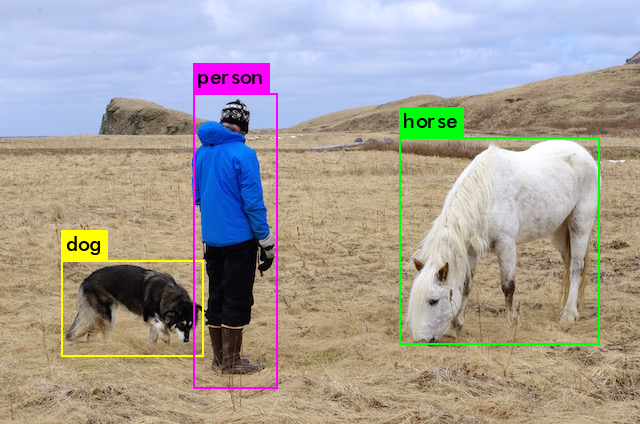
\includegraphics[width=12.5cm]{img/pred.png}
\caption{Sample Prediction Results from YOLOv2 Core}
\label{ml_demo}
\end{figure} 
 
Excluding weight loading times, the (unoptimized) demonstration program outputted the results featured above (Figure \ref{ml_demo}) in \textasciitilde 1.1 seconds.
 
 \section{Power Usage Test (\textit{T.P.1}) Results}\label{appendix:T.P.1}
 \begin{table}[H]
    \caption{Power Test Results}
	\centering
	\begin{tabular}{llll}
	\hline
	\textbf{Category} & \textbf{Voltage} & \textbf{Current} & \textbf{Power} \\
	\hline
    PLB --- idle & 12 V & 250 mA & 3 W\\
    PLB --- running testing program & 12 V & 400 mA & 4.8 W\\
    PMB --- idle & 5 V & 720 mA & 3.6 W\\
    PMB --- running video streaming application & 5 V & 840 mA & 4.2 W\\
    PMB --- full-load & 5 V & 1200 mA & 6 W\\
	\hline
	\end{tabular}
\end{table}
 \section{Battery Test (\textit{T.P.3}) Results}\label{appendix:T.P.3}
 \begin{table}[H]
	\centering
	\caption{Voltage reading}
	\begin{tabular}{ll}
	\hline
	\textbf{Time (minutes)} & \textbf{Voltage}\\
	\hline
    0 & 12.16V \\
    5 & 12.14V \\
    10 & 12.11V \\
    15 & 12.06V \\
    20 & 12.01V \\
    25 & 11.96V \\
    30 & 11.92V \\
	\hline
	\end{tabular}
\end{table}
\centering
After test battery level : \textbf{75\%}


% Content here

\end{document}